\section{\textsc{Eierkuchen}}

\subsection*{Zutaten für 2 Portionen:}

\begin{tabular}{p{7.5cm} p{7.5cm}}
	& \\
	100g Mehl & 40g Zucker \\
	300ml Milch & 4 Eier \\
	Prise Salz & Öl für die Pfanne \\
	\multicolumn{2}{l}{Puderzucker zum Dekorieren}
\end{tabular}

\subsection*{Serviervorschlag:}

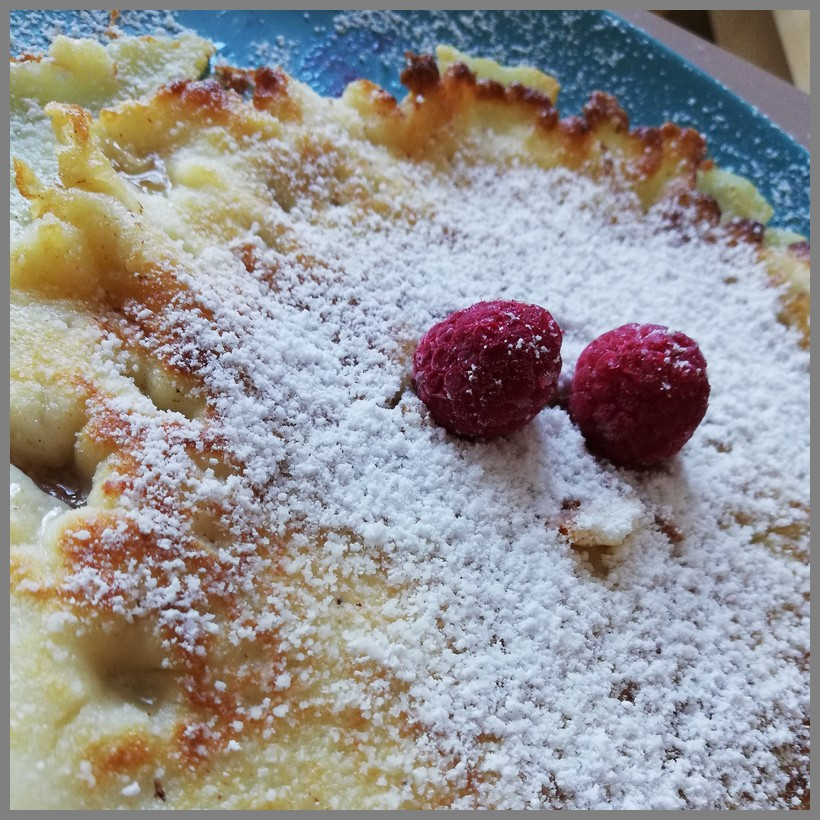
\includegraphics[width=\textwidth]{img/pancakes.jpg} \cite{pancakes}

\subsection*{So geht's:}

\begin{tabular}{p{15cm}}
	\\
	Die Eier trennen und das Eiweiß mit einem Schneebesen zu Eischnee schlagen.\\
	Den Zucker, die Milch, das Eigelb mit einer Prise Salz vermischen.\\
	Das Mehl in die Mischung sieben. Dadurch wir der Teig feiner.\\
	Nun den Eischnee langsam und sorgfältig unterheben, damit es nicht wieder zerfällt.\\
	Das Öl in einer Pfanne erhitzen. Zur Überprüfung die Rückseite eines Holzkochlöffels, oder einen Holzstab ins Öl halten. Schlägt das Öl Blasen, ist es heiß genug.\\
	Den Teig mit einer mittelgroßen Kelle in die Pfanne geben.\\
	Die Pfannkuchen nun auf beiden Seiten goldbraun anbraten.\\
	Mit Puderzucker bestreuen und heiß servieren.
\end{tabular}
